\documentclass[11pt]{article}

\usepackage{a4wide}
\usepackage{mathptm}
\usepackage{xspace}
\usepackage{amsmath}
\usepackage{graphicx}
\usepackage{algorithm}
\usepackage{algpseudocode}
\usepackage{tikz}
\usepackage{tkz-graph}
\usetikzlibrary{shapes.misc, positioning}
\usepackage{listings}
\usepackage{color}
\usepackage{hyperref}

\definecolor{dkgreen}{rgb}{0,0.6,0}
\definecolor{gray}{rgb}{0.5,0.5,0.5}
\definecolor{mauve}{rgb}{0.58,0,0.82}

\lstset{frame=tb,
  language=Java,
  aboveskip=3mm,
  belowskip=3mm,
  showstringspaces=false,
  columns=flexible,
  basicstyle={\small\ttfamily},
  numbers=left,
  numberstyle=\tiny\color{gray},
  keywordstyle=\color{blue},
  commentstyle=\color{dkgreen},
  stringstyle=\color{mauve},
  breaklines=true,
  breakatwhitespace=true,
  tabsize=3
}
\begin{document}

\title{My Best Software Technology Evaluation Project Ever}

\author{Some Student and Some other Student}

\maketitle

\begin{abstract}

  10-15 lines with the software technology and the highlights from the
  project that has been undertaken.

\end{abstract}

%\input{commands}

\section{Introduction}
\label{sec:introduction}


\subsection{Technology stack}
The primary objective of this project was to develop a prototype implementation of a web-based polling application.
This application allows users to create and participate in polls efficiently through a user-friendly interface. 
By leveraging web development frameworks and tools, the project aims to provide a robust and scalable platform for conducting polls.

To achieve this we made use of the following technology stack:

\begin{itemize}
    \item \textbf{Backend Framework and Language}
    \begin{itemize}
        \item Spring Boot with Kotlin
    \end{itemize}

    \item \textbf{Persistence Layer}
    \begin{itemize}
        \item Spring JPA  with database options PostgreSQL and MongoDB
    \end{itemize}

    \item \textbf{Frontend Framework}
    \begin{itemize}
        \item SvelteKit with Vite and TailwindCSS
    \end{itemize}

    \item \textbf{Messaging}
    \begin{itemize}
        \item Spring messaging with RabbitMQ
    \end{itemize}

    \item \textbf{Containerization and Deployment}
    \begin{itemize}
        \item Docker
    \end{itemize}
\end{itemize}


\subsection{Results}
The results obtained through this project highlight the feasibility and effectiveness of the proposed architecture with a usable website for running polls.
The prototype demonstrates key functionalities of the polling application, including poll creation, participation, and result aggregation.
Kotlin, in particular, proved advantageous for backend development, offering concise syntax and seamless integration with Java-based frameworks, which streamlined development and reduced boilerplate code.
The use of SvelteKit on the frontend ensures a responsive and engaging user experience, while the combination of Spring Boot, JPA and RabbitMQ in the backend provides a scalable and reliable infrastructure.
In addition, the inclusion of both relational and non-relational database options offers flexibility to cater to diverse use cases. \\

\subsection{Organization of report}
The remainder of this report is organized as follows:
\begin{itemize}
    \item \textbf{Section~\ref{sec:design}: Discusses the design of the application, outlining the design choices and user interface considerations.}
    \item \textbf{Section~\ref{sec:technology}: Evaluates Kotlin as a programming language for this project.}
    \item \textbf{Section~\ref{sec:implementation}: Delves into the prototype implementation, including frontend and backend.}
    \item \textbf{Section~\ref{sec:conclusion}: Concludes the report with a summary of findings and potential areas for future work.}
\end{itemize}


\section{Design}
\label{sec:design}
Around 5 pages about functional aspects of the FeedApp application.
Concretely, you shall write about 
\begin{itemize}
	\item the \emph{use cases},
	\item the \emph{domain model}, and
	\item the \emph{architecture} (including applied technologies)
\end{itemize}
Each part shall ideally be accompanied with a graphical representation (diagram).
You may have a look at the \href{https://github.com/selabhvl/dat250public/blob/master/projectdescription/README.md}{Examples on GitHub}.
In this section, we provide an overview of the functional aspects of the FeedApp application, focusing on the use cases, domain model, and architecture, including the technologies used in the backend, frontend, and messaging layers.
\begin{itemize}
    \item Source: \href{https://chatgpt.com/share/672fbc4f-ecf4-8007-b147-6759b1884b9c}{ChatGPT}
\end{itemize}
\subsection{Use Cases}
The FeedApp application provides a polling system where users can create, participate in, and manage polls. The key use cases are as follows:
\begin{itemize}
    \item \textbf{User Registration and Authentication:} Users can create an account, log in, and authenticate via email and password. This ensures that only registered users can create and vote in polls.
    \item \textbf{Poll Creation:} Authenticated users can create new polls by submitting a question and providing multiple voting options. Only registered users can create polls.
    \item \textbf{Vote on Polls:} Registered users can vote on available polls by selecting one of the options. Each user can vote only once per poll.
    \item \textbf{View Poll Results:} Users can view the current results of active polls, including the vote counts for each option.
    \item \textbf{Edit and Delete Polls:} Poll creators can edit or delete polls they have created, provided the poll is still open.
    \item \textbf{Vote Modification:} Users can modify their vote in an active poll.
    \item \textbf{Event Logging:} The system logs key events, such as vote casting, poll creation, and poll editing, for auditing and analytics purposes.
\end{itemize}
Each use case is supported by the backend services to ensure proper functionality, and the user interface provides a seamless experience for interacting with these actions.
\subsection{Domain Model}
The domain model of the FeedApp consists of several key entities that represent the core data objects of the system. These entities are mapped to the database and interact through the business logic.
\begin{itemize}
    \item \textbf{User:} Represents the users of the system. Each user has a unique identifier, email, password, and roles (admin, voter).
    \item \textbf{Poll:} Represents a poll created by a user. A poll has a unique identifier, a question, multiple options for voting, and a status (active, closed).
    \item \textbf{Vote:} Represents a vote cast by a user on a specific poll. A vote has a reference to the user who cast it, the poll being voted on, and the selected option.
    \item \textbf{Event:} Represents events logged in the system, such as vote events, poll creation events, and poll edit events. Events are tracked for auditing and analytics purposes.
\end{itemize}
The diagram above illustrates the relationships between the entities, with associations such as a user creating a poll, casting a vote, and generating events.
\subsection{Architecture and Applied Technologies}
The architecture of the FeedApp is designed to be modular and scalable, with separate services responsible for managing user data, polls, votes, and events. 
\begin{itemize}
    \item \textbf{Backend Framework and Language:} 
    \begin{itemize}
        \item \textbf{Spring Boot:} Used for building the backend API, providing RESTful endpoints for managing users, polls, and votes.
        \item \textbf{Kotlin:} Chosen for its concise syntax and interoperability with Java, making it a great fit for Spring Boot applications.
    \end{itemize}
    
    \item \textbf{Persistence Layer:} 
    \begin{itemize}
        \item \textbf{Spring JPA:} Used for database access with ORM (Object-Relational Mapping) support. Polls and votes are stored in PostgreSQL, while MongoDB is used for logging events.
        \item \textbf{PostgreSQL:} Relational database used to store user and poll data.
        \item \textbf{MongoDB:} Non-relational database used for storing event logs, providing scalability and flexibility for log data.
    \end{itemize}
    
    \item \textbf{Frontend Framework:} 
    \begin{itemize}
        \item \textbf{SvelteKit:} A modern frontend framework used for building fast, reactive web applications with minimal overhead.
    \end{itemize}
    
    \item \textbf{Messaging:}
    \begin{itemize}
        \item \textbf{RabbitMQ:} Used as a message broker to handle asynchronous communication between services. Events like votes and poll updates are sent to RabbitMQ for processing and tracking.
    \end{itemize}
    \item \textbf{Containerization and Deployment:} 
    \begin{itemize}
        \item \textbf{Docker:} The entire application, including the backend, frontend, and database, is containerized using Docker for easy deployment and scalability.
    \end{itemize}
\end{itemize}
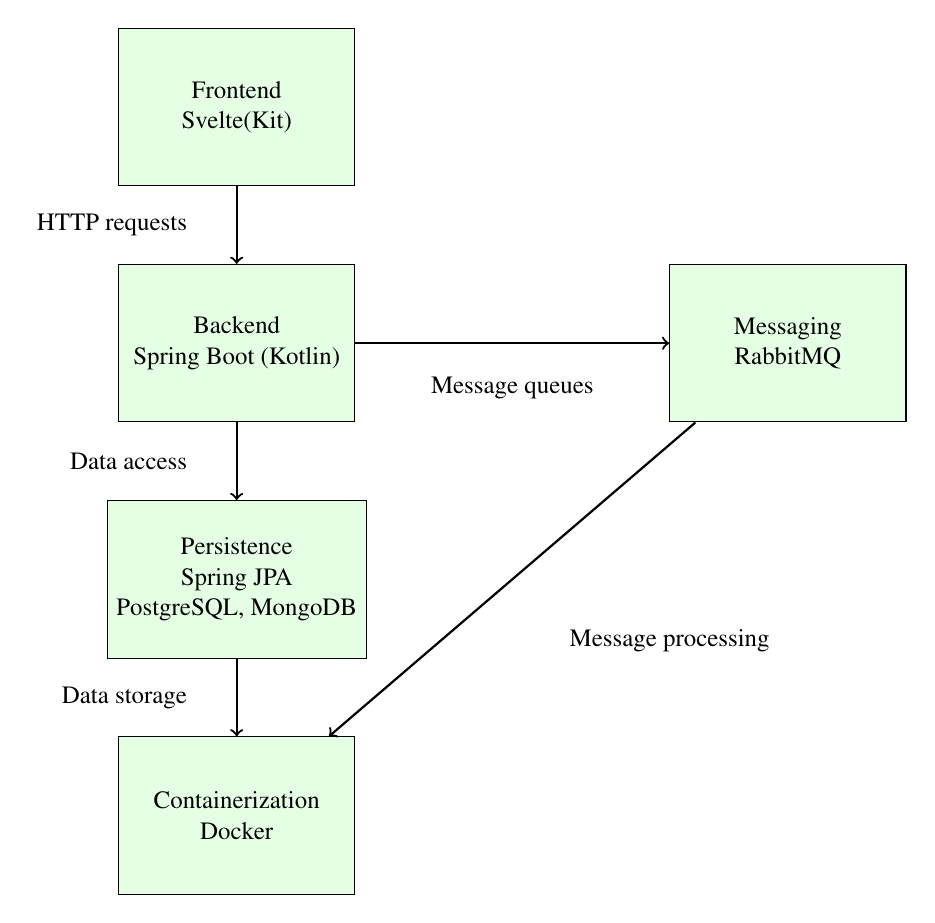
\begin{tikzpicture}[node distance=3cm, auto, font=\small]
    % Define the blocks for each component
    \node (frontend) [draw, rectangle, fill=green!10, text centered, minimum height=2cm, minimum width=3cm, align=center] {Frontend \\ Svelte(Kit)};
    \node (backend) [draw, rectangle, fill=green!10, below of=frontend, text centered, minimum height=2cm, minimum width=3cm, align=center] {Backend \\ Spring Boot (Kotlin)};
    \node (persistence) [draw, rectangle, fill=green!10, below of=backend, text centered, minimum height=2cm, minimum width=3cm, align=center] {Persistence \\ Spring JPA \\ PostgreSQL, MongoDB};
    \node (messaging) [draw, rectangle, fill=green!10, right of=backend, xshift=4cm, text centered, minimum height=2cm, minimum width=3cm, align=center] {Messaging \\ RabbitMQ};
    \node (container) [draw, rectangle, fill=green!10, below of=persistence, text centered, minimum height=2cm, minimum width=3cm, align=center] {Containerization \\ Docker};
    % Draw arrows to show the flow of interaction
    \draw[->, thick] (frontend) -- (backend) node[midway, left, xshift=-0.5cm] {HTTP requests};
    \draw[->, thick] (backend) -- (persistence) node[midway, left, xshift=-0.5cm] {Data access};
    \draw[->, thick] (backend) -- (messaging) node[midway, below, yshift=-0.3cm] {Message queues};
    \draw[->, thick] (persistence) -- (container) node[midway, left, xshift=-0.5cm] {Data storage};
    \draw[->, thick] (messaging) -- (container) node[midway, below, yshift=-0.5cm, xshift=2cm] {Message processing};
\end{tikzpicture}
\subsection{Backend}
We will now look into how the Kotlin code is organized. We use Kotlin with Spring Boot as the backend. The code is organized into three main services: EventService, PollService, and UserService. These handle the business logic. We also have class JwtService,  which provides token management for authentication.
 
\vspace{1cm}
\vspace{1cm}
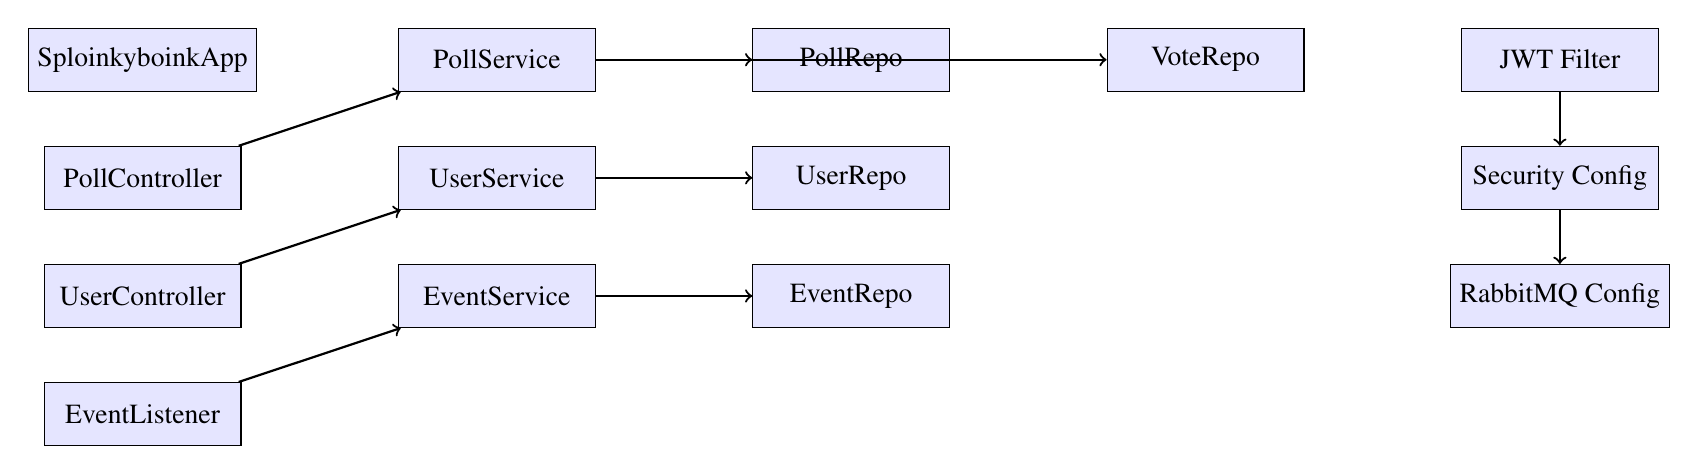
\begin{tikzpicture}[node distance=1.5cm]
% Define UML class styles
\tikzstyle{class} = [rectangle, draw=black, fill=blue!10, text centered, minimum height=0.8cm, minimum width=2.5cm]
\tikzstyle{arrow} = [->, thick, draw=black]
% Define nodes (classes)
\node[class] (SploinkyboinkApplication) {SploinkyboinkApp};
\node[class, below of=SploinkyboinkApplication] (PollController) {PollController};
\node[class, below of=PollController] (UserController) {UserController};
\node[class, below of=UserController] (EventListener) {EventListener};
% Define second layer nodes (Services)
\node[class, right of=SploinkyboinkApplication, xshift=3cm] (PollService) {PollService};
\node[class, below of=PollService] (UserService) {UserService};
\node[class, below of=UserService] (EventService) {EventService};
% Define third layer nodes (Repositories)
\node[class, right of=PollService, xshift=3cm] (PollRepository) {PollRepo};
\node[class, below of=PollRepository] (UserRepository) {UserRepo};
\node[class, below of=UserRepository] (EventRepository) {EventRepo};
\node[class, right of=PollRepository, xshift=3cm] (VoteRepository) {VoteRepo};
% Define fourth layer nodes (Security)
\node[class, right of=VoteRepository, xshift=3cm] (JwtAuthFilter) {JWT Filter};
\node[class, below of=JwtAuthFilter] (SecurityConfig) {Security Config};
% Define fifth layer nodes (Configurations)
\node[class, below of=SecurityConfig] (RabbitMQConfig) {RabbitMQ Config};
% Relationships (arrows)
\draw[arrow] (PollController) -- (PollService);
\draw[arrow] (UserController) -- (UserService);
\draw[arrow] (EventListener) -- (EventService);
\draw[arrow] (PollService) -- (PollRepository);
\draw[arrow] (PollService) -- (VoteRepository);
\draw[arrow] (UserService) -- (UserRepository);
\draw[arrow] (EventService) -- (EventRepository);
\draw[arrow] (JwtAuthFilter) -- (SecurityConfig);
\draw[arrow] (SecurityConfig) -- (RabbitMQConfig);
\end{tikzpicture}
\vspace{1cm}

\noindent \textbf{Main Application Class}
\begin{itemize}
    \item \textbf{SploinkyboinkApp}: The central class responsible for initializing and running the application.
\end{itemize}

\noindent \textbf{Controllers}
\begin{itemize}
    \item \textbf{PollController}: Manages HTTP requests related to polls.
    \item \textbf{UserController}: Handles user-related HTTP requests.
    \item \textbf{VoteController}: Processes vote-related HTTP requests.
    \item \textbf{EventListener}: Handles event-triggered actions.
\end{itemize}

\noindent \textbf{Services (Business Logic)}
\begin{itemize}
    \item \textbf{EventService}: Logs events such as user votes and poll creation/editing.
    \item \textbf{PollService}: Manages polls and voting logic.
    \item \textbf{UserService}: Handles user registration, authentication, and data operations.
    \item \textbf{VoteService}: Manages vote-related logic.
    \item \textbf{JwtService}: Provides JWT token management for authentication.
\end{itemize}

\noindent \textbf{Repositories (Data Access)}
\begin{itemize}
    \item \textbf{PollRepo}: Interacts with the database for poll-related data.
    \item \textbf{UserRepo}: Manages user data persistence.
    \item \textbf{VoteRepo}: Handles database operations for votes.
    \item \textbf{EventRepo}: Supports event-related data storage and access.
\end{itemize}

\noindent \textbf{Security and Messaging}
\begin{itemize}
    \item \textbf{Security Config}: Configures application-wide security settings and authentication mechanisms.
    \item \textbf{JWT Filters}: Ensures secure token-based authentication.
    \item \textbf{RabbitMQ Config}: Sets up RabbitMQ for message processing and event handling.
\end{itemize}

\vspace{0.5cm}
\noindent \textbf{Achieved functionalities}
\begin{itemize}
    \item \textbf{Polling Functionality}: Users can create, manage, and participate in polls, with their votes accurately captured and stored.
    \item \textbf{Event Tracking}: Tracks important user actions, enabling auditing or analytics.
    \item \textbf{User Management}: Ensures secure user authentication and management through validation mechanisms.
    \item \textbf{Integration with Messaging}: RabbitMQ integration supports a scalable, event-driven architecture, enabling the decoupling of services and enhancing overall application performance.
\end{itemize}

\section{Technology Assessment}
\label{sec:technology}

\subsection{Descriptive Modeling}

Kotlin, developed by JetBrains (the Czech software company behind IntelliJ IDEA), is named after Kotlin Island in the Gulf of Finland, near St. Petersburg. JetBrains introduced Kotlin in 2011 as a modern language addressing limitations encountered with Java. The first stable release (Kotlin 1.0) arrived in 2016 and gained traction among Android developers quickly. In 2017, Google endorsed Kotlin as an official language for Android development, a significant boost in adoption. In 2020, JetBrains and Google launched the Kotlin Foundation, solidifying its role in JVM and Android development. Kotlin’s ongoing development focuses on multi-platform capabilities, broadening its use beyond JVM and Android to include web, iOS, and server applications. Kotlin is a statically typed language that compiles to Java bytecode, running on the Java Virtual Machine (JVM), which allows compatibility with Java libraries and frameworks. Designed for safety, conciseness, and interoperability with Java, Kotlin is particularly valuable in three contexts:

\begin{itemize}
    \item \textbf{Android Development}: Kotlin’s concise syntax and enhanced safety features make it a preferred choice in Android development.
    \item \textbf{Server-Side Development}: Kotlin’s seamless integration with JVM-based frameworks like Spring Boot facilitates its use in server applications.
    \item \textbf{Multi-Platform Development}: Kotlin Multiplatform and Kotlin/Native enable shared codebases across platforms, including mobile, web, and desktop applications.
\end{itemize}

\begin{tikzpicture}[node distance=1.5cm]

\hspace*{-1.5cm}  % Shifts everything 1.5 cm to the left

% Define block styles
\tikzstyle{block} = [rectangle, rounded corners, minimum width=3cm, minimum height=1cm, text centered, draw=black, fill=blue!20]
\tikzstyle{problem} = [rectangle, rounded corners, minimum width=3cm, minimum height=1cm, text centered, draw=black, fill=red!20]
\tikzstyle{context} = [ellipse, minimum width=4cm, minimum height=1cm, text centered, draw=black, fill=yellow!20]
\tikzstyle{arrow} = [thick,->,>=stealth]
\tikzstyle{usecase} = [rectangle, rounded corners, minimum width=3.5cm, minimum height=1cm, text centered, draw=black, fill=green!20]

% Nodes
\node (problem1) [problem] {Problem 1: Verbose Code};
\node (problem2) [problem, below of=problem1] {Problem 2: Null Safety};
\node (problem3) [problem, below of=problem2] {Problem 3: Complex Asynchronous Code};
\node (context) [context, right of=problem2, xshift=4cm] {Context: Java Development};
\node (kotlin) [block, below of=context, yshift=-1cm, minimum width=4cm, minimum height=1.25cm, font=\large] {Kotlin};

% Spread out the blue boxes
\node (feature1) [block, below of=kotlin, xshift=-4cm] {Concise Syntax};
\node (feature2) [block, below of=kotlin] {Null Safety};
\node (feature3) [block, below of=kotlin, xshift=4cm] {Coroutines};

% Spread out the benefits
\node (benefit1) [block, below of=feature1] {Reduced Boilerplate};
\node (benefit2) [block, below of=feature2] {Enhanced Safety};
\node (benefit3) [block, below of=feature3] {Improved Concurrency};

% Use cases (stacked vertically)
\node (usecase1) [usecase, above of=context, xshift=6cm] {Android Development};
\node (usecase2) [usecase, below of=usecase1] {Server-Side Development};
\node (usecase3) [usecase, below of=usecase2] {Multi-Platform Development};

% Arrows
\draw [arrow] (problem1) -- (context);
\draw [arrow] (problem2) -- (context);
\draw [arrow] (problem3) -- (context);
\draw [arrow] (context) -- (kotlin);
\draw [arrow] (kotlin) -- (feature1);
\draw [arrow] (feature1) -- (benefit1);
\draw [arrow] (kotlin) -- (feature2);
\draw [arrow] (feature2) -- (benefit2);
\draw [arrow] (kotlin) -- (feature3);
\draw [arrow] (feature3) -- (benefit3);

% Arrows from use cases to context (yellow oval)
\draw [arrow] (usecase1) -- (context);
\draw [arrow] (usecase2) -- (context);
\draw [arrow] (usecase3) -- (context);

\end{tikzpicture}
\vspace{1cm}

\noindent \textbf{Key features of Kotlin}
\\
\noindent Kotlin is addressing some of Java's limitations. Kotlin as a programming language has many strengths:
\\
\textbf{Conciseness and Readability}: Kotlin’s streamlined syntax reduces repetitive code, improving readability and maintainability. This conciseness also minimizes potential sources of error and makes the codebase easier to work with.
\\
\textbf{Null Safety}: Kotlin’s type system helps prevent NullPointerExceptions by distinguishing between nullable and non-nullable types. This feature significantly reduces bugs related to null handling, a frequent issue in Java.
\\
\textbf{Asynchronous Programming with Coroutines}: Kotlin’s coroutines offer a simplified approach to asynchronous programming, enabling more efficient, non-blocking code execution ideal for network requests or tasks involving resource waits.
\\
\textbf{Interoperability with Java}: Kotlin’s full compatibility with Java allows teams to gradually integrate Kotlin into existing Java applications. This flexibility is advantageous for modernization efforts without requiring a complete code rewrite.
\\
\textbf{Multi-Platform Support}: Kotlin’s multiplatform capabilities allow for shared business logic across platforms, reducing code duplication and streamlining development for applications targeting Android, iOS, web, and server environments.
\\
\textbf{Functional Programming Features}: Kotlin includes extension functions, higher-order functions, and lambdas, allowing more expressive, modular code. These features support functional programming, further enhancing code flexibility and promoting cleaner architecture.
\\
\textbf{Data Classes}: Kotlin’s data classes simplify the creation of classes primarily used for holding data by automatically generating common methods like \texttt{equals()}, \texttt{hashCode()}, and \texttt{toString()}, streamlining data handling.


\subsection{Experiments: Is Kotlin bettter suited in developement than Java? }

In this section, we present a series of hypotheses regarding the potential benefits of using Kotlin over Java, along with experimental designs that could help validate or refute these assumptions. We are comparing Kotlin and Java code to see the differences between the languages. Some of the concepts discussed in the examples will also apply to our PollApp. 
\\
\\
\textbf{Hypothesis 1: Using Kotlin will provide better development speed and code conciseness than Java.} 
\\
\\
Kotlin’s syntax is designed to be more compact and expressive, which should reduce the time required to implement core functionalities such as user, poll, and vote management. To test this hypothesis, we can compare the time it takes to implement key features in both Kotlin and Java, while also measuring the number of lines of code required to achieve the same outcomes. We come up with a simple example for a class we call person, and compare the lines of code (LOC) to the same class implemented in Java. Our PollApp uses many classes, so a simple class structure is very beneficial:
\\
\\
\textbf{Experiment Example}:
\begin{tcolorbox}[colframe=blue!80!black, colback=blue!5!white, coltitle=blue!50!black, title={-}, boxrule=0.5mm, width=0.8\textwidth, sharp corners=south]
    \begin{itemize}
    \vspace{0.2cm}
        \item \textbf{\scriptsize Kotlin} (\scriptsize Data class):
        \begin{lstlisting}[style=kotlin, basicstyle=\scriptsize\ttfamily]
data class Person(val name: String, val age: Int)
        \end{lstlisting}
        
        \item \textbf{\scriptsize Java} (\scriptsize Full class):
        \begin{lstlisting}[style=java, basicstyle=\scriptsize\ttfamily]
public class Person {
    private String name;
    private int age;

    public Person(String name, int age) {
        this.name = name;
        this.age = age;
    }

    public String getName() { return name; }

    public int getAge() { return age; }

    @Override public String toString() { 
        return "Person{name='" + name + "', age=" + age + '}'; 
    }
}
        \end{lstlisting}
    \end{itemize}
\end{tcolorbox}
\vspace{1cm}

\noindent \textbf{Evaluation}: We see from the examples that Java are using significant more lines of code than Kotlin to achieve the same functionality. Kotlin uses only one line, while Java uses 17 lines of code when we include the empty lines in between. This is a significant difference. Kotlin's \texttt{data class} reduces the need for boilerplate code (like getters, setters, and \texttt{toString()}), making the code more concise and error-resistant. Java’s verbose approach introduces potential for mistakes and increases the overall code length. Hypothesis 1 holds. 
\\
\\
\textbf{Hypothesis 2: Using Kotlin will result in fewer runtime exceptions related to null pointer errors compared to Java.} 
\\
\\ 
We will provide a small example that highlights why Java are more prone to null pointer errors than Kotlin. Null pointer errors can happen in situations where entities like users, polls, or votes do not exist even though they are expected to. These kinds of errors are common in Java, where null checks must be manually implemented. To evaluate this, we could introduce null values in critical parts of the business logic (e.g., missing users or votes) and compare the frequency of runtime exceptions between Kotlin and Java. By observing how each language handles missing data, we can assess Kotlin’s ability to enhance application stability. We will not test this in our project, but it is good to know that there are more ways to test the null safety of different programming languages.
\\
\\
\begin{tcolorbox}[colframe=blue!80!black, colback=blue!5!white, coltitle=blue!50!black, title={-}, boxrule=0.5mm, width=0.8\textwidth, sharp corners=south]
    \begin{itemize}
    \vspace{0.2cm}
        \item \textbf{\scriptsize Kotlin} (\scriptsize Null safety):
        \begin{lstlisting}[style=kotlin, basicstyle=\scriptsize\ttfamily]
fun greet(name: String?) {
      println("Hello, ${name ?: "Guest"}!")
}
greet(null)  // Output: Hello, Guest!
        \end{lstlisting}
        
        \item \textbf{\scriptsize Java} (\scriptsize Manual null check):
        \begin{lstlisting}[style=java, basicstyle=\scriptsize\ttfamily]
public void greet(String name) {
        if (name == null) {
            name = "Guest";
        }
        System.out.println("Hello, " + name);
}
greet(null);  // Output: Hello, Guest!
        \end{lstlisting}
    \end{itemize}
\end{tcolorbox}

\noindent \textbf{Evaluation}: From the examples we see that Kotlin is designed so that it does not need to handle null checks manually. Kotlin’s \texttt{null} safety ensures that nullability is explicitly handled using \texttt{?} and \texttt{?:}, reducing runtime errors. Java’s manual null checks are error-prone and can be easily missed, leading to potential \texttt{NullPointerException} risks. Hypothesis 2 holds.
\\
\\
\textbf{Hypothesis 3: Kotlin's coroutines offer a more efficient, responsive, scalable and readable approach to handling asynchronous tasks compared to Java.}
\\
\\ 
To validate this hypothesis, we present an example demonstrating the use of Kotlin coroutines and Java threads for handling asynchronous tasks. While we did not implement this exact feature in our PollApp, it highlights the potential benefits of using coroutines in scenarios involving high concurrency, like handling voting requests. In a different testing scenario, we would compare Kotlin’s coroutine-based voting logic with a similar Java implementation using traditional threads. We would simulate high traffic and track key metrics such as response time and memory usage to evaluate scalability under load. We use this example because it shows us very concretely how concurrency is managed in a simple way. 
\\
\\
\\
\textbf{Experiment Example}:

\begin{tcolorbox}[colframe=blue!80!black, colback=blue!5!white, coltitle=blue!50!black, title={-}, boxrule=0.5mm, width=0.8\textwidth, sharp corners=south]
    \begin{itemize}
    \vspace{0.2cm}
        \item \textbf{\scriptsize Kotlin} (\scriptsize Null Coroutines):
        \begin{lstlisting}[style=kotlin, basicstyle=\scriptsize\ttfamily]
import kotlinx.coroutines.*

suspend fun fetchData() {
    delay(1000)
    println("Data fetched")
}

fun main() = runBlocking {
    launch { fetchData() }
}
        \end{lstlisting}
        
        \item \textbf{\scriptsize Java} (\scriptsize Threads):
        \begin{lstlisting}[style=java, basicstyle=\scriptsize\ttfamily]
public class Main {
    public static void fetchData() {
        try {
            Thread.sleep(1000);
            System.out.println("Data fetched");
        } catch (InterruptedException e) {
            e.printStackTrace();
        }
    }

    public static void main(String[] args) {
        Thread thread = new Thread(() -> fetchData());
        thread.start();
    }
}
        \end{lstlisting}
    \end{itemize}
\end{tcolorbox}

\noindent \textbf{Evaluation}: Kotlin coroutines simplify asynchronous code, making it more readable and reducing boilerplate code. Java’s thread-based approach requires more code and is harder to manage due to explicit thread handling and synchronization. Coroutines are lightweight, allowing many concurrent tasks with minimal memory usage, whereas Java threads consume more resources. Coroutines scale efficiently since they are managed by a dispatcher and don't block threads, resulting in faster response times compared to Java threads, which block during operations like Thread.sleep(). Additionally, coroutines are simpler to manage and more readable than Java threads, making them a more efficient choice for asynchronous data handling in performance-sensitive applications. Hypothesis 3 holds.

\vspace{1em}

\noindent \textbf{Hypothesis 4: Kotlin's extension functions enable developers to write cleaner, more modular, and reusable code compared to Java.}

\vspace{1em}

\noindent To test this hypothesis, we compare how Kotlin and Java handle extending the functionality of an existing class, such as adding a method to capitalize the first letter of a string. Kotlin achieves this through extension functions, while Java requires either inheritance or a utility class.

\vspace{1em}

\noindent \textbf{Experiment Example:}  

\begin{tcolorbox}[colframe=blue!80!black, colback=blue!5!white, coltitle=blue!50!black, title={-}, boxrule=0.5mm, sharp corners=south, top=5mm, bottom=5mm, left=5mm, right=5mm]
    \begin{minipage}[t]{0.48\textwidth}
        \raggedright
        \textbf{\scriptsize Kotlin} (\scriptsize Using Extension Functions)
        \vspace{0.2cm}  % Extra space between header and code
        \begin{lstlisting}[style=kotlin, basicstyle=\fontsize{4}{5}\ttfamily, frame=none]
fun String.capitalizeFirstLetter(): String {
    return this.replaceFirstChar { it.uppercase() }
}

fun main() {
    val text = "kotlin is fun"
    println(text.capitalizeFirstLetter())  // Output: "Kotlin is fun"
}
        \end{lstlisting}
    \end{minipage}%
    \hfill
    \begin{minipage}[t]{0.48\textwidth}
        \raggedright
        \textbf{\scriptsize Java} (\scriptsize Using a Utility Class)
        \vspace{0.2cm}  % Extra space between header and code
        \begin{lstlisting}[style=java, basicstyle=\fontsize{4}{5}\ttfamily, frame=none]
public class StringUtils {
    public static String capitalizeFirstLetter(String input) {
        if (input == null || input.isEmpty()) return input;
        return input.substring(0, 1).toUpperCase() + input.substring(1);
    }
}

public class Main {
    public static void main(String[] args) {
        String text = "java is powerful";
        System.out.println(StringUtils.capitalizeFirstLetter(text));  // Output: "Java is powerful"
    }
}
        \end{lstlisting}
    \end{minipage}
\end{tcolorbox}

\vspace{1em}

\noindent \textbf{Evaluation:}  
The Kotlin approach allows the method to be called directly on the \texttt{String} object as if it were part of the class, improving readability and making the code feel more natural. In Java, a separate utility class is required, leading to a more cumbersome and less intuitive syntax. Additionally, Kotlin’s solution integrates seamlessly with the language’s functional programming features. Kotlin's extension functions make code more modular and intuitive by enabling developers to add functionality to existing classes without modifying them or creating external helper classes. This reduces boilerplate and enhances code reusability. Hypothesis 4 holds. 

\vspace{1em}

\noindent \textbf{Hypothesis 5: Kotlin has seamless interoperability with Java in addtition to better features.}

\vspace{1em}

\noindent In this case, we choose to provide a code example demonstrating Kotlin's ability to directly use Java libraries and classes without additional configuration. In the previous examples we have shown how Kotlin has better features than Java. Kotlin's interoperability allows developers to leverage the extensive Java ecosystem while benefiting from Kotlin's concise syntax and null safety features. If we were to test this hypothesis, we would compare the ease of using a popular Java library in both Java and Kotlin. Key metrics such as code readability, development speed, and error prevention would be analyzed. The Kotlin example in this case uses the java library to import Hash Map.

\vspace{1em}

\noindent \textbf{Experiment Example}:

\begin{tcolorbox}[colframe=blue!80!black, colback=blue!5!white, coltitle=blue!50!black, title={-}, boxrule=0.5mm, width=0.8\textwidth, sharp corners=south]
    \begin{itemize}
        \item \textbf{\scriptsize Kotlin}:
        \begin{lstlisting}[style=kotlin, basicstyle=\scriptsize\ttfamily]
    import java.util.HashMap

    fun main() {
        // Using Java's HashMap class in Kotlin
        val map = HashMap<String, Int>()
        map["Apples"] = 5
        map["Oranges"] = 3

        // Using null-safe operations
        println(map["Apples"] ?: "No apples found")
        println(map["Bananas"] ?: "No bananas found")
    }
        \end{lstlisting}
    \end{itemize}
\end{tcolorbox}

\vspace{1em}

\noindent \textbf{Evaluation}: The Kotlin example demonstrates how Java libraries can be used directly, with benefits like null-safe operations (\texttt{?:} operator) and concise syntax. Kotlin's integration with Java's mature ecosystem, supported by resources and community, enhances its practicality for real-world applications.  Kotlin’s interoperability with Java simplifies migration and allows developers to leverage the strengths of both languages effectively. Hypothesis 5 holds. 


\vspace{1em}

\subsection{Experiment Evaluation}

Through these experiments, we can assess the various advantages Kotlin offers over Java. 
\vspace{1em}

\noindent \textbf{Comparison Table}

\vspace{1em}

\begin{table}[ht]
\centering
\resizebox{\textwidth}{!}{ % Resize the table to fit the page width
\begin{tabular}{|>{\raggedright\arraybackslash}p{2.5cm}|>{\raggedright\arraybackslash}p{3.5cm}|>{\raggedright\arraybackslash}p{3.5cm}|>{\raggedright\arraybackslash}p{3.0cm}|>{\raggedright\arraybackslash}p{3.5cm}|}
\hline
\textbf{Feature}            & \textbf{Kotlin Advantage}                 & \textbf{Java Approach}            & \textbf{Key Metrics}           & \textbf{Result}                          \\ \hline
Concise Syntax              & Data classes reduce boilerplate          & Requires manual getters/setters   & Lines of Code (LOC)      & Kotlin reduced LOC from 17 to 1 \\ \hline
Null-Safety                    & Type system enforces null handling       & Relies on manual null checks      & Null Pointer Exceptions (NPE) & Kotlin eliminated potential NPEs \\ \hline
Coroutines                    & Better handling of asynchronous code & Thread-based model            & Memory Usage, Response Time, Scalability  &  Kotlin had readable and efficient coroutines for handling concurrency \\ \hline
Standard Library           & Built-in utilities (e.g., \texttt{let}, \texttt{apply}) & Requires external libraries     & Developer Effort (subjective) & Kotlin provided simpler, cleaner code \\ \hline
Java Ecosystem Access & Seamless library integration             & Native use                       & Ecosystem Compatibility      & Kotlin leveraged HashMap from the Java.util library \\ \hline
\end{tabular}
}
\caption{Comparison of Kotlin and Java}
\label{tab:comparison}
\end{table}


\vspace{1em}

\noindent \textbf{Final Conclusion}: Kotlin stands out as a modern, practical language that enhances developer productivity and system efficiency. Its concise syntax minimizes boilerplate, while its built-in null-safety ensures greater reliability by preventing runtime errors. Coroutines enable highly efficient, scalable concurrency, making it well-suited for handling large volumes of concurrent tasks. Additionally, Kotlin’s rich standard library simplifies common operations, and its full interoperability with Java ensures seamless integration with existing ecosystems. These strengths make Kotlin an excellent choice for both new projects and for modernizing existing codebases.


\end{document}




\section{Prototype Implementation}
\label{sec:implementation}

This section should provide brief details of how the prototype has been implemented.
You may want to use come code snippets here, but only focus on core features and aspects.
You are not meant to copy/paste your whole application code into the report.
Focus for instance how other developers may run your application and how they might develop it further...


The example below shows how you may include code. There are similar
styles for many other langages - in case you do not use Java in your
project. You can wrap the listing into a figure in case you need to
refer to it. How to create a figure was shown in Section~\ref{sec:technology}.

\lstinputlisting[language=java]{code/BoksVolum.java}



\section{Conclusions}

Concludes on the project, including the technology, its maturity,
learning curve, and quality of the documentation.

The references used throughput the report should constitute a well
chosen set of references, suitable for someone interesting in learning
about the technology.


\bibliographystyle{plain}
\bibliography{report.bib}{}

\end{document}
